\documentclass[11pt,a4paper]{article}
\usepackage[T1]{fontenc}
\usepackage[utf8]{inputenc}
\usepackage[margin=25mm]{geometry}
\usepackage{lmodern}
\usepackage{amsmath,amssymb}
\usepackage{graphicx}
\usepackage{booktabs,tabularx,array}
\usepackage{xcolor}
\usepackage{microtype}
\usepackage{url}
\usepackage[hidelinks]{hyperref}
\usepackage{caption}
\captionsetup{font=small,labelfont=bf}
\setlength{\emergencystretch}{2em}
\setlength{\parskip}{0.3em}
\setlength{\tabcolsep}{5pt}
\renewcommand{\arraystretch}{1.12}
\graphicspath{{figures/}}
\newcommand{\code}[1]{\texttt{\detokenize{#1}}}
\newcommand{\unit}[1]{\,\mathrm{#1}}

\title{Toward SDN-Controlled Microgrid Reconfiguration:\\
An Auditable Python--PSCAD Switching Testbed}
\author{Author Names to Be Confirmed\\
\small Department and Institution to Be Confirmed\\
\small Corresponding Author Email to Be Confirmed}
\date{Research manuscript draft -- 5 September 2026}

\begin{document}
\maketitle
\begin{abstract}
Separating network-control development from electrical-model development is
useful for studying programmable feeder restoration, but a graph-valid route
alone does not establish its electrical behavior. This paper presents an
SDN-inspired Python--PSCAD testbed that translates structured controller
commands into timed low-voltage breaker operations, executes an electromagnetic
transient experiment, and returns traceable measurements to a graphical
dashboard. The implementation retains the networking simulator separately from
the power-plane integration and preserves JSON as the exchange contract beneath
graphical editing. A six-bus, seven-branch, 400-V feeder with two normally open
ties provides the initial electrical case. A read-only analysis of six saved
PSCAD experiments examines baseline operation, isolation, restoration, loop
rejection, imposed control delay, and a native three-phase-to-ground fault.
In the physical-fault case, the maximum absolute phase current is 1.554 kA;
healthy downstream buses recover to 380.5--387.4 V after approximately 1.195 s
below a 200-V analysis threshold, while the faulted bus remains isolated.
The contribution is an auditable command-to-EMT workflow and its preliminary
functional evidence, not a new optimal reconfiguration algorithm or a
demonstration of real-time closed-loop SDN protection. Illustrative electrical
parameters, non-transactional command handling, and the absence of live
controller feedback delimit the results and motivate the next validation stage.
\end{abstract}

\noindent\textbf{Keywords:} software-defined networking; low-voltage feeder;
microgrid reconfiguration; PSCAD; electromagnetic transients; reproducibility.

\section{Introduction}
Distribution feeder reconfiguration changes which sectionalizing and tie
switches conduct, allowing the same physical infrastructure to supply loads
through different connected configurations. Classical work treats this as an
electrical-network problem with objectives such as loss reduction and load
balancing \cite{baran1989}. Software-defined networking (SDN), by comparison,
separates programmable forwarding decisions from the mechanisms that execute
them in a communication network \cite{mckeown2008}. The conceptual separation
is attractive for a project in which one team develops network-control logic
and another investigates physical low-voltage (LV) switching.

The analogy has an important boundary. Alternating-current power is not
forwarded as independently addressed packets through passive feeder branches.
Switching alters circuit connectivity, after which voltages and currents follow
the network impedances, source characteristics, and electrical dynamics.
Consequently, a route returned by a networking algorithm must be translated
into a physically represented switching sequence and evaluated in an
electrical simulator. A graph can establish connectivity; it cannot, by
itself, establish acceptable voltage, equipment loading, transient behavior,
or protection coordination.

The broader project aims to maintain a communication control plane independently
of switchable power paths. Its present electrical realization is a single-source
LV feeder, not a complete multi-resource microgrid. This distinction matters:
the U.S. Department of Energy's microgrid description includes local energy
resources, controllability as an entity, and grid-connected or islanded
operation \cite{doeMicrogrids}. The current case has neither distributed
energy resource (DER) control nor a demonstrated islanding transition. The
term ``toward'' in the title therefore denotes a research trajectory rather
than an already validated operating capability.

This paper asks three practical questions. First, can externally specified
network commands be mapped consistently onto physical breaker schedules while
retaining identifiers and operation-level decisions? Second, do the saved EMT
measurements show the expected distinction between fault inception, isolation,
and restoration of healthy loads? Third, can graphical dashboard edits trigger
fresh, inspectable PSCAD experiments without changing the networking team's
implementation?

The resulting contributions are:
\begin{enumerate}
\item A modular command-to-power-plane workflow that retains a structured
controller contract, operation-level graph checks, explicit component bindings,
and a reproducible timed experiment manifest.
\item A PSCAD automation path with native breaker and fault components,
serialized run ownership, fresh-result checks, and a defined set of 31 research
channels exposed through a graphical JSON-backed dashboard.
\item An evidence-bounded analysis of six saved deterministic scenarios,
including a physical fault, downstream restoration, and an explicitly imposed
restoration delay, accompanied by reproducible publication assets.
\end{enumerate}
These are integration and functional-validation contributions. No superiority
over established reconfiguration algorithms or cyber-physical testbeds is
claimed. The experiments support further research on the interface between
network decisions and electrical consequences; they are not evidence that
the proposed architecture is ready to operate a physical feeder.

\section{Background and Related Work}
\subsection{Electrical Reconfiguration and Software-Defined Control}
Baran and Wu formulated distribution reconfiguration in terms of electrical
losses and load balance, establishing the relevance of switch state and radial
network structure \cite{baran1989}. The present work uses radiality only as an
operation-level topological constraint. It does not implement their optimization
procedure, solve an optimal power flow, or benchmark a new route-selection
method.

OpenFlow provides an influential example of a programmable interface between
network control and forwarding elements \cite{mckeown2008}. Applying this idea
to an energy system requires care over which plane is being programmed. In
conventional SDN, the data plane forwards communication traffic. In the project
terminology, the ``power plane'' instead denotes conducting electrical paths;
the interface described here is not an OpenFlow implementation for breakers.

Software-defined microgrid control is already an established research topic.
Wang et al. virtualize microgrid control functions as software services,
reducing dependence on dedicated controller hardware \cite{wang2020}. Li and
Du employ SDN and OpenFlow to support programmable communications for networked
microgrid formation, partition, and reconfiguration \cite{li2021}. These works
preclude a broad novelty claim that separating control from physical microgrid
operation is itself new. The narrower focus here is retaining an evolving
network-team command contract while producing an inspectable PSCAD switching
experiment and measurement record.

\subsection{Communications and Cyber-Physical Simulation}
Communication behavior can influence control outcomes, but a delayed timestamp
is not equivalent to a simulated communication network. Dorsch et al. compare
legacy and software-defined communications in distributed smart-grid control,
explicitly considering communication infrastructure and agent interaction
\cite{dorsch2017}. The long-delay case in this paper instead imposes a later
restoration time. It illustrates the electrical cost of waiting, without
measuring packet loss, routing convergence, or SDN latency.

Federated simulators address a different problem from batch automation. FNCS
couples power-system and communication simulators with synchronization
strategies for their exchanges \cite{ciraci2014}. HELICS supports coordinated
event-driven and time-series simulations, including iteration among federates
\cite{palmintier2017}. Neither framework is integrated into the current
implementation. Their relevance is methodological: a persistent application
connection does not supply the shared-time and causality mechanisms required
for closed-loop co-simulation.

More recent cyber-physical emulation also extends well beyond scheduled
switching. Haque et al. combine an operational-microgrid-derived power model
with a synthetic communication network, DNP3 exchanges, and structured threat
scenarios \cite{haque2025}. Their work provides a useful contrast to the
illustrative feeder and deterministic commands used here; this paper makes
no comparative cybersecurity or resilience-performance claim.

\begin{table}[tb]
\centering\small
\caption{Positioning against selected related work. Entries describe scope,
not a ranking or a feature-completeness assessment.}
\label{tab:related}
\begin{tabularx}{\textwidth}{@{}p{32mm}XX@{}}
\toprule
Work & Principal emphasis & Distinction of this study \\
\midrule
Baran--Wu \cite{baran1989} & Electrical reconfiguration objectives & Evaluates supplied routes; no optimizer \\
Wang et al. \cite{wang2020} & Virtualized microgrid controllers & Command-to-EMT experiment integration \\
Li--Du \cite{li2021} & SDN-enabled networked microgrids & JSON batch interface, not live OpenFlow \\
FNCS / HELICS \cite{ciraci2014,palmintier2017} & Synchronized simulator federation & Sequential automation of a single EMT run \\
Haque et al. \cite{haque2025} & Cyber-physical threat emulation & Illustrative switching and fault scenarios \\
\bottomrule
\end{tabularx}
\end{table}

\subsection{PSCAD as the Electrical Execution Layer}
PSCAD exposes Python automation for loading and running projects
\cite{pscadAutomation}. Its timed breaker component supports one or two
operations associated with a breaker control signal \cite{pscadTimedBreaker}.
The supplied fault models represent a fault using switched resistances rather
than a detailed arc characteristic \cite{pscadFaults}. These documented
facilities are sufficient for the deterministic switching cases examined here.
The project-specific contribution lies in translating commands, managing run
completion and result freshness, and connecting the results to research
artifacts; it is not a replacement for the underlying EMT solver.

\section{System Architecture and Command Semantics}
\label{sec:architecture}
\subsection{Ownership Boundaries and Data Flow}
The original networking simulator remains in its existing repository modules.
The power-plane extension is housed separately under
\code{research_power_plane}, with dedicated command adaptation, topology,
timeline, PSCAD mapping, automation, measurement, and dashboard modules.
This separation allows networking colleagues to evolve their algorithms while
the adapter handles changes in their output fields. It does not guarantee
compatibility with an arbitrary future schema: new aliases and semantic changes
must be tested at the adapter boundary.

Figure~\ref{fig:architecture} shows the implemented workflow. A controller
output batch or a graphical dashboard submission supplies topology, commands,
optional faults, and logical-to-PSCAD bindings. Canonical JSON remains the
exchange representation. The dashboard provides feeder selection, switch-state
controls, scheduled operations, fault forms, and mapping tables; advanced raw
JSON remains available. Committing an edit can automatically invoke the same
pipeline as a command-line replay. Selecting an element or moving the
scheduled-state preview is not a simulation request.

\begin{figure}[tb]
\centering
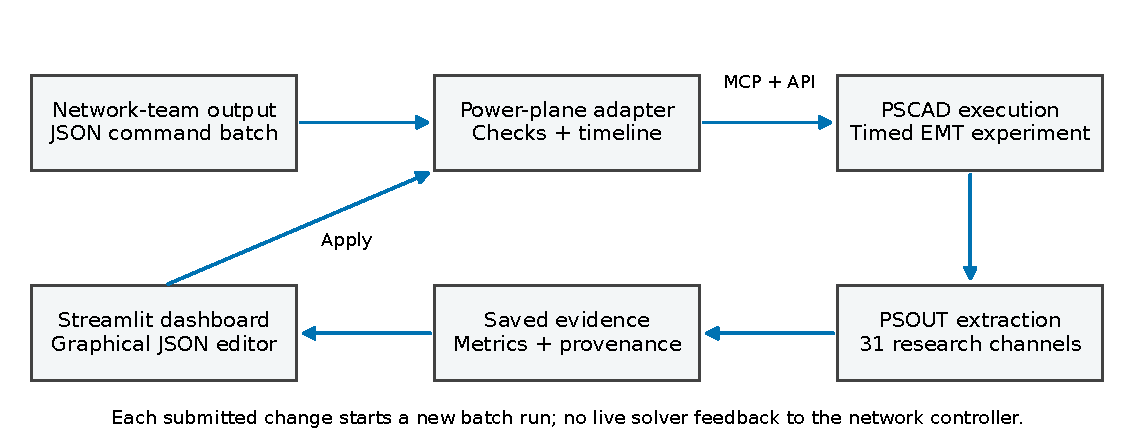
\includegraphics[width=\textwidth]{architecture.pdf}
\caption{Implemented batch workflow. Solid arrows indicate current processing
paths. Measurement display follows run completion; no feedback path from the
running EMT solver to the networking controller is implemented.}
\label{fig:architecture}
\end{figure}

The displayed network state and the PSCAD wiring are related but not
interchangeable. The present dashboard operates on the fixed six-bus electrical
case and its component map. A new graph edge without a corresponding wired
PSCAD branch does not create a new physical circuit. Extending the feeder
requires an electrical-model and mapping update.

\subsection{Command Contract and Graph Model}
Represent a normalized command as
\begin{equation}
 c_k = (\mathrm{id}_k,\,\tau_k,\,a_k,\,\mathcal{O}_k,\,\mathcal{M}_k),
\end{equation}
where $\tau_k$ is a simulation-time timestamp, $a_k$ is an action,
$\mathcal{O}_k$ contains target nodes, edges, or a requested path, and
$\mathcal{M}_k$ holds controller identity and metadata. Supported actions
include opening or closing a line, isolating or restoring a node, applying
a switch set, and requesting a reroute path. Commands are processed in a
stable chronological order, retaining input order for equal timestamps.

Let the physical connectivity model be the undirected graph
$\mathcal{G}=(\mathcal{V},\mathcal{E})$, with $x_e=1$ for a logically closed
branch and $x_e=0$ for an open branch. The currently conducting graph is
\begin{equation}
 \mathcal{G}_x = (\mathcal{V},\{e\in\mathcal{E}:x_e=1\}).
\end{equation}
For a source set $\mathcal{S}$, the software's energized-node estimate is the
union of connected components containing a source. This is a connectivity
estimate, not a voltage calculation. Likewise, the analysis field called
``island count'' counts connected components; it does not establish viable
grid-forming operation within a separated component.

With radiality preservation enabled and an initially acyclic graph, a proposed
closure $e=(u,v)$ is rejected if a path already connects $u$ and $v$ in
$\mathcal{G}_x$. Opening an edge cannot introduce a cycle. This local rule
preserves a forest during accepted edge changes, but does not require every
load to remain connected. It also does not enforce voltage limits, branch
ratings, source capacity, protection selectivity, or synchronization between
multiple sources.

An implementation detail limits the strength of the validation guarantee.
The current command handler records command-level warnings while processing
individual requested operations. A command may therefore be marked
unaccepted or partially accepted after some valid edge operations have already
been applied. Only accepted state-changing operations enter the switching
timeline; rejected operations and no-ops do not. This is
\emph{not an atomic, all-or-nothing transaction}. The loop-rejection experiment
tests a single rejected closure, not general rollback behavior. A production
interlock would require validation of the complete prospective transition
before committing it.

\subsection{Schedule Compilation and Execution}
Each logical line identifier maps to a PSCAD timed-logic component and its
associated three-phase breaker. The component's control convention reverses
the graph variable:
\begin{equation}
 b_e(t)=1-x_e(t),\qquad b_e=0\text{ closed},\quad b_e=1\text{ open}.
\label{eq:polarity}
\end{equation}
The adapter writes the initial state and operation count and times using
\code{INIT}, \code{NUMS}, \code{TO1}, and \code{TO2}. The current mapping
permits at most two transitions per breaker during one run, consistent with
the selected timed component \cite{pscadTimedBreaker}. An unchanged branch
receives an operation beyond the simulation window to accommodate the
component's lack of a zero-operation setting. The generated waveform inside
the experiment window remains constant.

Execution uses a project-local wrapper around PowerMCP, a Model Context
Protocol (MCP) server exposing PSCAD automation tools. A persistent localhost
service owns the application connection. The local wrapper focuses the intended
case and uses a blocking project run so that returning control means the run
has completed. The persistence avoids reopening the application for every
dashboard action; it does not represent an independently powered,
always-available field control network.

The client serializes project parameter writes with a run lock. To avoid the
PSCAD output-overwrite dialog, it removes only the current case's generated
output before building. Other case files and separately named archives are
preserved. Successful execution requires acceptable build messages, a newly
produced output fingerprint, and the expected measured channels. Tool errors,
missing channels, or stale results fail the request rather than being presented
as a successful new simulation.

These are engineering safeguards, not a formal proof of end-to-end correctness.
In particular, clearing the current raw output means that publication-grade
reproducibility needs a separate immutable archive for every run. Each new
submission starts another continuous EMT experiment from its specified initial
conditions. The current system does not alter a running simulation in response
to newly arriving controller messages.

\section{Electrical Test System}
\label{sec:model}
\subsection{Feeder and Load Representation}
The generated case, \code{SEIAN_LV_Timed_Switching}, comprises buses G01 and
N02--N06, seven three-phase switchable series R/L branches, and five balanced
Y-connected resistive loads. G01 is supplied by a Thevenin source configured
at 0.4 kV line-to-line RMS and 50 Hz, with a source resistance setting of
$0.02\unit{\Omega}$. The declared source setting and implemented branch values
are illustrative; they are not a short-circuit calibration against a measured
transformer or utility supply.

Five branches form the initial radial tree; N02--N05 and N04--N06 are normally
open ties. Opening N02--N03, N03--N04, and N03--N05 isolates N03. Closing both
ties then supplies the healthy downstream buses through
G01--N02--N05--N06--N04, as shown in Figure~\ref{fig:feeder}.

\begin{figure}[tb]
\centering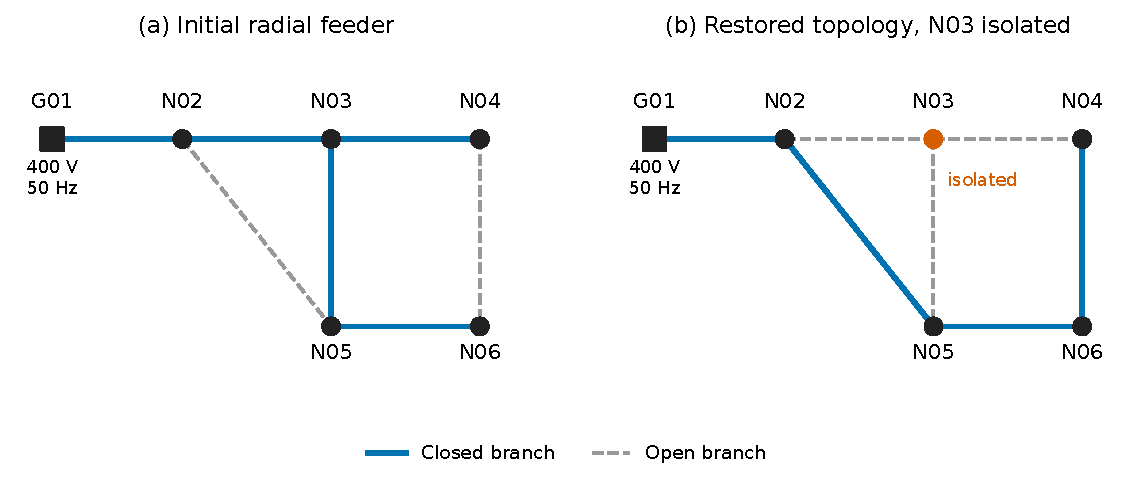
\includegraphics[width=\textwidth]{feeder.pdf}
\caption{Original schematic of the modeled electrical connectivity before and
after restoration. Lines represent three-phase branches, not communication
links or geographical cable routing. Node positions are diagrammatic.}
\label{fig:feeder}
\end{figure}

\begin{table}[tb]
\centering\small
\caption{Implemented per-phase branch parameters, extracted from the saved
PSCAD build report. These values are illustrative, not measured cable data.}
\label{tab:lines}
\begin{tabular}{@{}lrrl@{}}
\toprule
Branch & $R_e$ ($\Omega$) & $L_e$ ($\mu$H) & Initial state \\
\midrule
G01--N02 & 0.05000 & 47.75 & Closed \\
N02--N03 & 0.07500 & 71.62 & Closed \\
N03--N04 & 0.08571 & 81.85 & Closed \\
N05--N06 & 0.10000 & 95.49 & Closed \\
N03--N05 & 0.10000 & 95.49 & Closed \\
N02--N05 & 0.12000 & 114.59 & Open (tie) \\
N04--N06 & 0.12000 & 114.59 & Open (tie)
\\
\bottomrule
\end{tabular}
\end{table}

The builder assigns resistance from a nominal branch-capacity field. For a
numerical capacity entry $q_e$ in kW, its heuristic is
\begin{equation}
 R_e = \frac{3}{q_e}\unit{\Omega},\qquad
 L_e = \frac{0.3R_e}{2\pi f},\qquad f=50\unit{Hz}.
\end{equation}
The constant 3 is an implementation sizing heuristic with the implied unit
conversion, not a conductor law. Consequently, \code{capacity_kw} should
not be interpreted as an enforced thermal rating. Table~\ref{tab:lines}
reports the actual generated impedances directly.

The loads require similarly careful interpretation. The source builder
contains a scalar named \code{LOAD_PF}, set to $0.98$, but uses it to multiply
the target active power when calculating resistance. It does not introduce a
reactive load or enforce a 0.98 electrical power factor. If $P_i^{\mathrm{set}}$
is expressed in watts and $V_{LL,0}=400\unit{V}$, the implemented phase
resistance is
\begin{equation}
 R_{i,\phi}=
 \frac{(V_{LL,0}/\sqrt{3})^2}{0.98 P_i^{\mathrm{set}}/3}
 =\frac{V_{LL,0}^{2}}{0.98 P_i^{\mathrm{set}}}.
\label{eq:load}
\end{equation}
Thus the nominal-voltage resistive demand is $0.98P_i^{\mathrm{set}}$ and
varies approximately with the square of applied balanced RMS voltage. These
are not constant-power loads. Table~\ref{tab:loads} records both the original
sizing labels and the resulting nominal-voltage demands.

\begin{table}[tb]
\centering\small
\caption{Resistive load sizing. The demand column refers to 400-V operation,
not the measured demand at the loaded bus voltage.}
\label{tab:loads}
\begin{tabular}{@{}lrrr@{}}
\toprule
Bus & Sizing label (kW) & Demand at 400 V (kW) & $R_{i,\phi}$ ($\Omega$) \\
\midrule
N02 & 8 & 7.84 & 20.40816 \\
N03 & 8 & 7.84 & 20.40816 \\
N04 & 10 & 9.80 & 16.32653 \\
N05 & 8 & 7.84 & 20.40816 \\
N06 & 6 & 5.88 & 27.21088
\\
\bottomrule
\end{tabular}
\end{table}

\subsection{Fault and Numerical Configuration}
The physical-fault scenario uses a native three-phase-to-ground fault at N03,
with an on-resistance of $0.05\unit{\Omega}$ and an off-resistance of
$10^6\unit{\Omega}$. Its programmed inception is 4.8 s, duration 0.4 s,
and clearing time 5.2 s. All incident N03 breakers are commanded open at
5.0 s and both ties close at 6.0 s. Fault activation uses the native
\code{tpflt} and \code{tfaultn} components; it is not synthesized by manually
changing a plotted voltage trace. Finite off-resistance produces small leakage
when the fault is inactive. The native resistive-switch abstraction does not
model fault-arc dynamics \cite{pscadFaults}.

PSCAD advances the EMT solution with a $25\unit{\mu s}$ time step and records
research signals every $50\unit{\mu s}$. A duration-$T$ experiment therefore
contains $T/(50\unit{\mu s})+1$ recorded samples per channel when both endpoints
are included. Startup is included in the saved trajectories but excluded from
the interruption metric as described below. Time-step convergence, frequency
dependence of line parameters, grounding calibration, unbalanced demand,
inverter dynamics, and transformer detail have not been established for this
case.

\section{Experimental Method and Evidence Handling}
\label{sec:methods}
\subsection{Saved Scenario Matrix}
The evaluation is a read-only analysis of existing experiment artifacts,
frozen for manuscript preparation on 5 September 2026. No new PSCAD
simulations were launched while producing the paper. There is one saved
deterministic result per matrix condition, so no confidence interval,
stochastic reliability estimate, or repeated-run performance distribution is
reported.

The six conditions are: S1, no-fault baseline; S2, N03 isolation at 5 s without
restoration; S3, the same isolation followed by tie closure at 6 s; S4, attempted
closure of a tie that would create a loop in the initial topology; S5, isolation
at 5 s and deliberately delayed tie closure at 45 s; and S6, a native fault
at 4.8--5.2 s with isolation at 5 s and restoration at 6 s. S2 and S3 retain
``fault'' terminology in some originating filenames or scenario descriptions,
but contain only logical isolation commands, not an applied physical fault.
Only S6 energizes the native fault component.

The input reason string in S6 refers to protection detecting a fault. This is
scenario annotation, not evidence of a simulated detector. Both fault timing
and controller timing are provided in advance in the same experiment input.
The 0.2-s interval between fault inception and isolation is imposed; it does
not measure relay decision time or communication delay.

\begin{table}[tb]
\centering\footnotesize
\caption{Saved experiment matrix. Accepted commands are shown as accepted/issued.
Events count individual breaker transitions. The N04 duration is time below
200 V; $\geq$ marks an interval still ongoing when the run ended.}
\label{tab:scenarios}
\begin{tabularx}{\textwidth}{@{}lXrrrrr@{}}
\toprule
ID & Condition & Run (s) & Cmd. & Events & Samples/ch. & N04 (s) \\
\midrule
S1 & Baseline & 1 & 0/0 & 0 & 20,001 & 0.0000 \\
S2 & Isolation only & 6 & 1/1 & 3 & 120,001 & $\geq 0.9835$ \\
S3 & Tie restoration & 7 & 2/2 & 5 & 140,001 & 0.9984 \\
S4 & Loop rejection & 6 & 0/1 & 0 & 120,001 & 0.0000 \\
S5 & Delayed restoration & 46 & 2/2 & 5 & 920,001 & 39.9984 \\
S6 & Physical fault & 7 & 2/2 & 5 & 140,001 & 1.1948
\\
\bottomrule
\end{tabularx}
\end{table}

\subsection{Measured Channels and Interruption Metric}
Each run provides six bus RMS voltage channels in kV; seven branch RMS-current
channels in kA; seven branch active-power channels in MW; seven breaker-control
state channels; three instantaneous fault-current channels in kA; and one
fault-state channel. These sum to 31 research channels. The binary
\code{State_*} channels record scheduled control signals, not independent
mechanical-contact feedback. The fault-state signal uses 1 for active,
unlike the breaker convention in Equation~\ref{eq:polarity}.

The raw output also contains animation-related traces. The existing reader
distinguishes the research recorders from sparsely sampled display channels
instead of treating every exported trace as a full-rate measurement. The saved
integration evidence reports 146 raw traces and 31 selected research traces.

For recorded bus RMS voltage $V_i[n]$, define a threshold indicator
\begin{equation}
 z_i[n]=\begin{cases}
 1,& t_n\geq 0.5\unit{s}\ \text{and}\ V_i[n]<0.2\unit{kV},\\
 0,&\text{otherwise}.
 \end{cases}
\end{equation}
An interval begins at the first below-threshold sample and ends at the first
sample no longer below threshold. The implemented analysis merges consecutive
intervals separated by at most 0.02 s, then discards intervals shorter than
0.01 s. If an interval continues to the last sample, the saved duration is
right-censored at the run end. For each retained interval $j$,
\begin{equation}
 D_{i,j}=t_{i,j}^{\mathrm{end}}-t_{i,j}^{\mathrm{start}}.
\end{equation}
Because of the merge rule, $D_{i,j}$ can include very short recovered gaps;
it is a sustained-interruption envelope, not necessarily the exact integral of
$z_i$. The threshold is 0.5 per unit of the nominal 400-V voltage, chosen for
this experiment. It is not a claim of compliance with a voltage-quality
standard, nor a customer reliability index such as SAIDI.

The peak absolute current for fault phase $\phi$ is
\begin{equation}
 I_{\phi}^{\mathrm{pk}}=\max_n |i_{\phi}[n]|.
\end{equation}
The pipeline computes peaks and threshold intervals from the full recorded
series before reducing the displayed traces. Sample alignment is
$50\unit{\mu s}$; this spacing is not a calibrated accuracy bound on RMS
filter dynamics or switching-device behavior.

\subsection{Provenance and Visualization}
The source result file stores final values, extrema, event-aligned samples,
interruption metrics, and a 501-point evenly indexed preview per channel.
The manuscript script verifies channel counts, sample counts, preview order,
finite values, final-value consistency, and interval arithmetic against this
snapshot. It does not reconstruct full-rate waveforms from those previews.
The numerical tables use stored full-rate summaries; the plotted voltage and
RMS-current trajectories use explicitly labeled decimated previews.

In particular, evenly subsampled instantaneous fault current can alias the
50-Hz waveform and miss a peak. The paper therefore presents fault-current
peak bars from the saved full-rate metrics rather than inventing a detailed
waveform between preview points. Publication-grade transient waveform figures
will require separately archived raw outputs.

Provenance includes the inspected repository revision, SHA-256 hashes of the
read input artifacts and relevant source modules, the electrical build report,
and the scenario inputs. A recorded graphical-validation artifact supplies
additional evidence for baseline selection, physical-fault selection, and a
command edit through the dashboard. This evidence is reported as an earlier
integration check, not a new GUI experiment conducted during manuscript
preparation.

\section{Results}
\label{sec:results}
\subsection{Baseline, Isolation, and Loop Rejection}
All six saved matrix runs report 31 research channels, zero build errors, and
zero build warnings. The recorded sample counts match their respective
simulation durations at the specified output interval
(Table~\ref{tab:scenarios}). This is evidence of successful case execution and
recorder extraction, not proof that the parameter set is physically calibrated.

In S1, the downstream final RMS voltages range from approximately 382.0 to
386.97 V at N03--N06. The normally open tie currents are negligible, and no
retained below-threshold interval is reported. S2 opens the three incident
branches of N03 at 5 s. N03--N06 then remain below the analysis threshold to
the 6-s run end. N04 first crosses below 200 V at 5.0165 s, giving an observed
duration of 0.9835 s. This is only a lower bound on the unresolved
interruption, not a recovery time.

S4 rejects the single loop-forming closure and produces no state-changing
switching events. Its final voltage profile remains consistent with the
baseline. This establishes the intended behavior for that particular cycle
test. It does not establish atomic rejection for a mixed command containing
both acceptable and unacceptable operations.

\subsection{Tie Restoration and Imposed Delay}
In S3, tie closure at 6 s restores N04, N05, and N06 while N03 stays isolated.
The respective final voltages are 380.51, 387.37, and 383.43 V
(Table~\ref{tab:voltages}). The final tie currents are 32.54 A on N02--N05
and 13.45 A on N04--N06. These current magnitudes provide electrical evidence
that the alternate branches carry load after closure, beyond a graphical
indication that an edge is closed. They do not establish a thermal margin
against measured cable ratings.

\begin{table}[tb]
\centering\small
\caption{Saved final bus RMS voltage (V). The small N03 residual after
restoration is not usable service; finite off-state paths remain in the model.}
\label{tab:voltages}
\begin{tabular}{@{}lrrr@{}}
\toprule
Bus & S1 baseline & S3 restoration & S6 physical fault \\
\midrule
N03 & 386.97 & 0.02 & 0.02 \\
N04 & 384.83 & 380.51 & 380.51 \\
N05 & 383.51 & 387.37 & 387.37 \\
N06 & 382.03 & 383.43 & 383.43
\\
\bottomrule
\end{tabular}
\end{table}

N04 and N06 remain below 200 V for approximately 0.9984 s in S3, and N05 for
0.99805 s. In S5, changing the tie-closure time from 6 to 45 s increases each
of these saved interval durations by 39 s; their final voltage values remain
the same to the displayed precision. The difference is the direct consequence
of the imposed restoration schedule. It cannot be described as an SDN speedup
over a measured legacy network, because neither network-delay distribution nor
communications implementation is varied in these runs.

\begin{table}[tb]
\centering\small
\caption{Completed downstream intervals below 200 V, from saved full-rate
metrics. Displayed decimal places reflect sample-based accounting rather than
physical calibration accuracy.}
\label{tab:interruptions}
\begin{tabular}{@{}lrrr@{}}
\toprule
Bus & S3 duration (s) & S5 duration (s) & S6 duration (s) \\
\midrule
N04 & 0.99840 & 39.99840 & 1.19485 \\
N05 & 0.99805 & 39.99805 & 1.19455 \\
N06 & 0.99840 & 39.99840 & 1.19495
\\
\bottomrule
\end{tabular}
\end{table}

\subsection{Native Physical Fault and Restoration}
The physical-fault scenario produces a different voltage trajectory from
isolation-only switching. The fault input is active from 4.8 to 5.2 s;
N03--N06 cross below threshold around 4.820 s, before the scheduled breaker
opening at 5 s. The maximum absolute fault phase currents are 1.552, 1.554,
and 1.552 kA for A, B, and C, respectively. The largest recorded phase peak
is 1.554333 kA. In contrast, inactive-fault cases exhibit approximately
1.3 mA maximum leakage rather than a high-current event.

Opening the three N03 incident branches removes the source-fed route to the
fault location. The fault logic clears at 5.2 s, and the healthy downstream
buses are reconnected through the two ties at 6 s. Their below-threshold
durations are 1.19485 s at N04, 1.19455 s at N05, and 1.19495 s at N06.
Their final voltages and tie currents agree with S3 at the reported precision.
N03 remains isolated to the 7-s run end, with only a small residual measured
voltage. Restoring healthy loads therefore does not imply restoration of the
faulted bus.

\begin{figure}[tb]
\centering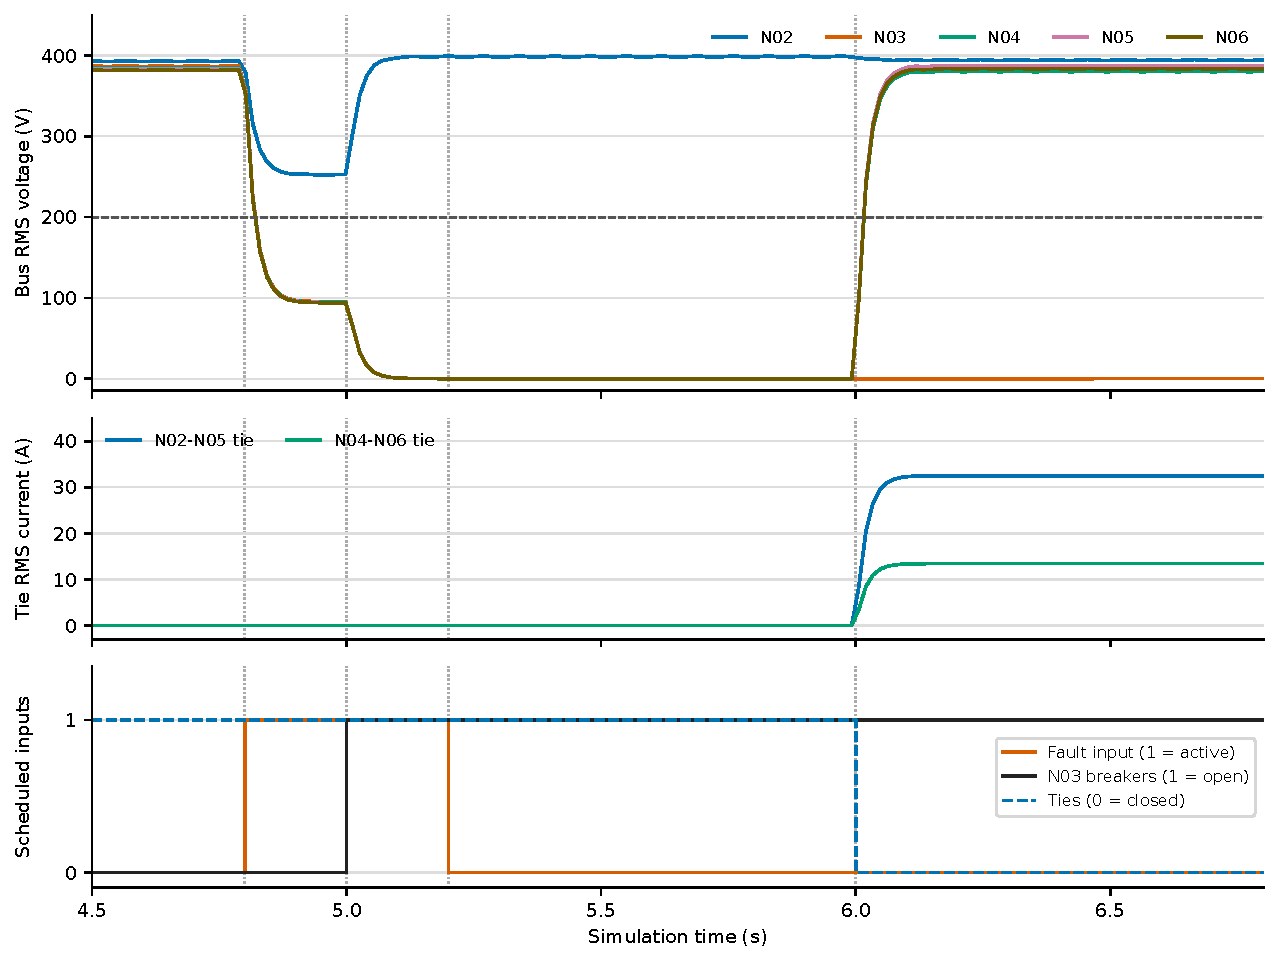
\includegraphics[width=0.96\textwidth]{physical_fault.pdf}
\caption{S6 physical-fault response near the switching events. The upper two
panels use the stored 501-point voltage and RMS-current previews from a
140,001-sample-per-channel run; they are decimated trajectories, not full-rate
transient waveforms. The lower panel shows exact input schedules, not measured
breaker-contact feedback. Dotted lines mark 4.8, 5.0, 5.2, and 6.0 s.}
\label{fig:physical}
\end{figure}

Figure~\ref{fig:physical} combines the stored RMS trajectories with the exact
scenario input schedule. Figure~\ref{fig:comparison} reports the interval
durations and fault-current peaks from the stored full-rate metrics. The
roughly 15--20 ms difference between a programmed transition and an RMS
threshold crossing should not be interpreted as communication latency. It
includes the voltage measurement's response and the electrical transient, as
well as the threshold definition.

\begin{figure}[tb]
\centering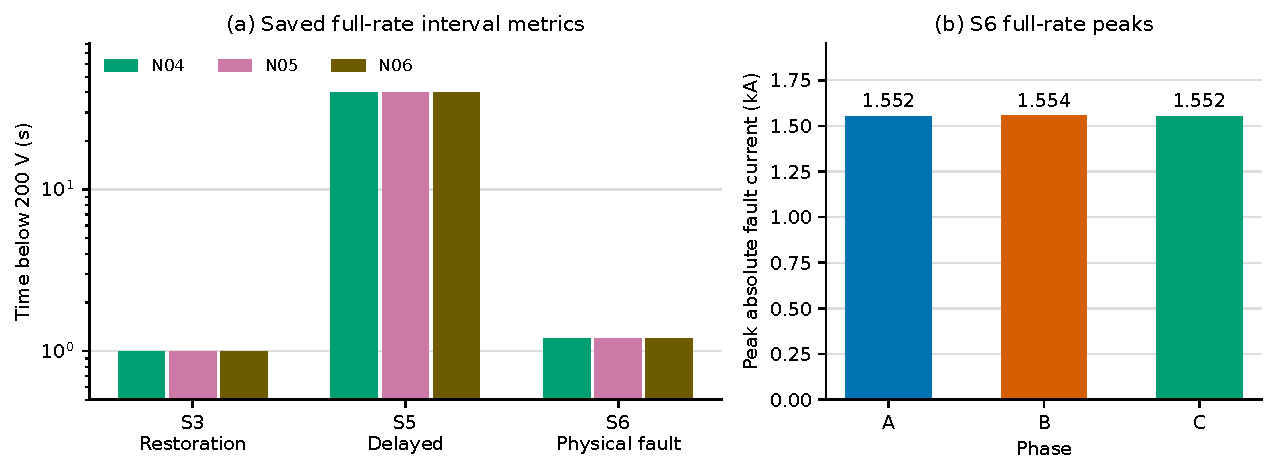
\includegraphics[width=\textwidth]{comparison.pdf}
\caption{Saved full-rate summary metrics. Panel (a) uses a logarithmic duration
axis to show the intentionally imposed long wait in S5 alongside S3 and S6.
Panel (b) reports phase-current peaks for S6; no peaks are estimated from
decimated waveform previews.}
\label{fig:comparison}
\end{figure}

\subsection{Recorded Dashboard Integration Evidence}
The graphical-validation artifact dated 5 September 2026 records three
successful actions: selecting the baseline, selecting the physical fault, and
editing a controller command. All three retain the same PSCAD process
identifier and return 31 selected channels with no reported errors. The
baseline has 20,001 samples per channel; both fault-related runs have 140,001.
The baseline fault-current peak is approximately $1.26\times10^{-6}$ kA,
while the phase-A peak for the physical-fault runs is approximately 1.552 kA.
The command-edit validation moves isolation from 5.0 to 5.1 s while retaining
the 6.0-s restoration time and the same fixed feeder model.

Together with the parameter manifests and fresh-output checks, this evidence
supports the implemented dashboard-to-PSCAD batch workflow. It is not a
measurement of end-to-end dashboard latency, proof of uninterrupted control
connectivity, or a live feedback demonstration. The project context also
records 114 passing automated tests; those tests were not rerun for this
read-only manuscript task and are not counted as additional experiments.

\section{Discussion, Limitations, and Research Agenda}
\label{sec:discussion}
\subsection{What the Evidence Establishes}
The saved artifacts show consistency across three representations: a requested
network action, the accepted operation-level schedule, and the resulting
electrical measurements. The isolation-only and physical-fault cases separate
two phenomena that a purely graphical demonstration might conflate.
Disconnecting a bus is not itself a short circuit; the native fault case
adds an independently scheduled conductive path and measured fault current.
Similarly, tie closure is supported by measured branch current and downstream
voltage recovery, not just a changed line color.

The workflow is useful as a collaboration boundary. Networking colleagues can
provide candidate routes without becoming responsible for PSCAD component
identifiers, while electrical-model development can proceed without rewriting
their routing code. The operation and measurement records make disagreements
inspectable: a missing graph path, rejected closure, invalid mapping, failed
build, stale output, and an electrically poor result are different failure
classes. This separation supports debugging and subsequent experimental design.

Nevertheless, traceability is not equivalent to electrical admissibility.
Radiality and source connectivity are necessary modeling checks for the chosen
scenario, but they are not a complete operating envelope. An overload or
unacceptable voltage may occur in an acyclic, source-connected network. A
future controller must use calibrated electrical constraints and independent
interlocks before these commands could be considered for hardware.

\subsection{Threats to Validity}
\paragraph{Electrical validity.}
The six-bus network is intentionally small and uses illustrative branch
impedances, source settings, and resistive loads. The load-sizing scalar is
not the load power factor, and demand is voltage dependent. There is no
validated transformer, grounding arrangement, DER controller, switching arc,
protection curve, or grid-forming island. The restored voltage range should
not be generalized to a campus or community microgrid without a new parameter
set and validation.

\paragraph{Control and safety semantics.}
The implemented route checks are local and operation based. Partial command
execution is possible, and command warnings are not equivalent to a
transactional abort. This is a material limitation for generalizing the
loop-rejection result. Atomic validation, explicit safe intermediate states,
independent permissives, and rollback or recovery policies should precede
any live or hardware-facing controller integration.

\paragraph{Timing and communications.}
No independent communication failure is simulated in the electrical run.
The control delay is an input, not an observed transport characteristic.
An always-connected control-plane objective remains untested, including its
power supply, redundancy, reconnection behavior, and failure isolation.
The MCP service is a local automation mechanism, not a safety-rated
field protocol or evidence of secure, reliable network delivery.

\paragraph{Measurement and repeatability.}
The analysis threshold and interval filtering are experimental definitions.
The selected breaker-state traces are controller outputs rather than
independent contacts. The stored 501-point previews cannot support detailed
fault-waveform reconstruction. No timestep-convergence study, independently
recomputed per-scenario raw-output analysis, repeated-run variance, or
instrument calibration is supplied with this draft. The saved deterministic
matrix supports functional inspection, not statistical reliability claims.

\paragraph{Novelty and comparison.}
Software-defined microgrids and cyber-physical testbeds already exist. The
current manuscript does not show that its automation architecture outperforms
those systems, or that the networking algorithm is optimal. A future venue
submission must align its contribution with an appropriately scoped systems
or experimental-methods claim, or add a genuinely new and evaluated control
method.

\subsection{Next Experimental Stage}
The next stage should first freeze measured or benchmark electrical
parameters, validate the steady state and fault level independently, and
repeat the cases at multiple EMT time steps. A larger feeder and unbalanced
loads would test whether the adapter remains useful beyond the current
balanced six-bus example. Branch ampacity, source limits, neutral and grounding
models, and load dynamics should be explicit inputs rather than inferred from
network-capacity labels.

Live integration then needs an agreed controller transport with versioned
messages, identifiers, acknowledgments, stale-command handling, and a
well-defined failure policy. Fault detection must originate from measured
electrical signals if the experiment is to evaluate protection response.
Closing the measurement-to-controller loop also requires an explicit clock
and synchronization strategy; established federation approaches such as
HELICS and FNCS provide relevant design precedents
\cite{palmintier2017,ciraci2014}, but choosing or integrating one is future
work.

A useful comparative protocol would hold the electrical case fixed and vary
only the controller and communication treatment. Candidate conditions are
manual or fixed restoration, the current supplied-route policy, and the
networking team's updated policy. Controlled delay, loss, disconnection, and
recovery distributions should use documented seeds and repeated trials.
Record detection time, issue time, receipt time, breaker operation, and load
recovery separately; do not collapse them into a single ``SDN delay.''

The evaluation should report operation-level and transaction-level rejection,
voltage-limit violations, loading limits, switching count, recovery duration,
and unavailable demand. For example, a future energy-not-served measure could
be defined using a specified counterfactual demand trajectory:
\begin{equation}
 E_{\mathrm{NS}}=\sum_i\int
 \max\{P_i^{\mathrm{required}}(t)-P_i^{\mathrm{served}}(t),0\}\,dt.
\end{equation}
This metric is not computed here. In a resistive-load model, reduced consumed
power during undervoltage is not automatically equivalent to disconnected
customer demand; the counterfactual must be stated before calculating such
an index. Comparative results should include uncertainty appropriate to the
randomized treatments and retain all raw electrical and communication logs.

\section{Conclusion}
This paper describes a working batch interface from structured network-control
commands and graphical dashboard edits to timed PSCAD electrical experiments.
The modular implementation preserves the networking code boundary while
linking logical identifiers, operation-level decisions, component parameters,
fresh outputs, and measured results. Six saved deterministic scenarios provide
preliminary functional evidence for baseline operation, isolation, tie-based
restoration, single-loop rejection, imposed waiting time, and a native
three-phase fault.

In the physical-fault case, a maximum absolute phase current of 1.554 kA
precedes restoration of healthy downstream buses to approximately
381--387 V, with about 1.195 s below the selected 200-V threshold. The faulted
bus stays isolated. These observations support the command-to-EMT workflow,
not a claim of optimal routing, measured SDN latency, or completed live
microgrid protection. Calibrated models, atomic command semantics, independent
fault detection, and synchronized controller feedback are the principal
requirements for the next research stage.


\section*{Data and Code Availability}
The manuscript package contains a frozen extract of the existing six-scenario
results, scenario inputs, electrical build metadata, provenance hashes,
generated figures, and the scripts used to produce its tables and plots.
It does not contain a complete per-scenario archive of raw PSCAD output.
The originating networking repository is
\url{https://github.com/MathishaBuwaneka/SEIAN-AMRP-Mesh-Simulator}.
That URL identifies the upstream networking work; it is not a claim that the
local power-plane extension or this manuscript has been publicly released there.
The availability and licensing of a submission-time research release remain
to be confirmed by the authors.

\section*{Author and Funding Statements}
Author order, affiliations, individual contributions, acknowledgments, funding,
and competing-interest declarations must be completed by the project team
before submission. No external funding or deployment authorization is asserted
in this draft.

\bibliographystyle{unsrt}
\bibliography{references}
\clearpage
\appendix
\section{Reproducibility and Artifact Guide}
\label{sec:reproducibility}
The independent manuscript package generates its numerical tables and four
original figures from a frozen saved-result snapshot. Its generator neither
launches PSCAD nor writes into operational folders. Snapshot refresh is an
explicit, read-only access to the source project.

\begin{table}[h]
\centering\small
\caption{Manuscript-package contents and their evidential role.}
\begin{tabularx}{\textwidth}{@{}p{64mm}X@{}}
\toprule
Artifact & Role \\
\midrule
\code{data/evidence_snapshot.json} & Saved scenario results, input batches, electrical metadata, and GUI-validation summary \\
\code{data/provenance.json} & Original input hashes, snapshot time, and inspected repository revision \\
\code{data/scenario_summary.csv} & Numeric values underlying the six-scenario table \\
\code{scripts/prepare_artifacts.py} & Read-only evidence extraction and figure/table generation \\
\code{figures/}, \code{tables/} & Generated manuscript assets \\
\code{research_notes.md} & Literature source audit, claim boundaries, and author checklist \\
\code{build.ps1} & Local LaTeX and BibTeX build into the paper's build directory \\
\bottomrule
\end{tabularx}
\end{table}

The inspected repository revision is
\code{7db42ae0e9f8092065cf77bb206b1a818c29eacd}.
This identifies the revision present when the artifacts were read, not a
verified build-time commit for every historical experiment. Individual SHA-256
hashes identify the actual inputs used by the manuscript. The existing
project context records PSCAD 5.0.1 Educational, Python 3.13.7,
\code{mhi.pscad} 2.9.7, \code{mhi.psout} 1.3.0, PowerMCP 0.3.0,
MCP 2.1.1, Streamlit 1.63.0, and Playwright 1.62.0. These are recorded local
versions, not a complete environment lock or a claim of compatibility across
other installations. PSCAD licensing and a compatible compiler remain
requirements for independently rerunning the electrical experiments.

The source workspace is \path{research_power_plane/pscad_workspace}.
Its principal evidence files are \code{transient_scenario_results.json},
\code{timed_feeder_build_report.json}, and
\path{validation/graphical_gui_validation.json}.
Source modules governing the principal claims are
\code{power_plane.py} (per-operation acceptance), \code{timeline.py}
(state-changing schedules), \code{pscad_adapter.py} (component mapping),
\code{pscad_mcp_client.py} and \code{pscad_mcp_server.py} (execution),
and \code{transient_analysis.py} (metric definitions).

\paragraph{Rebuild the paper.}
Run the optional artifact generator and then the PDF build from this folder:
\begin{quote}\small\ttfamily
py -B scripts/prepare\_artifacts.py\\
.\textbackslash build.ps1
\end{quote}
Only artifact generation needs Python, Matplotlib, and NumPy. The document
uses the conventional \code{article} class and BibTeX; no online service or
venue-specific template is required.

\paragraph{Reproduce the science.}
Rebuilding tables does not reproduce the EMT experiments. A scientific release
must additionally archive the exact case and component library, compiler and
dependency versions, initialization, command and fault manifests, per-scenario
\code{.psout} files, solver messages, and rerunnable analysis. Archive each raw
output before another run replaces it. Author and venue review is necessary
before public release.

\end{document}
